Global existence of a solution to the wave equation with a quadratic non-linearity fails on $\R_t \times \R^3_x$. For example, it was shown in \cite{john1981} that every solution with smooth compactly supported initial data to 
	\[ \Box \phi = \partial_t \phi \partial_t \phi\]
exhibits finite-time blow-up. Nevertheless, by imposing restrictions on the non-linearity, we can recover the desired decay. The key observation is that for such non-linear waves, not all derivatives decay at the same rate.

\subsection{Controlling ``good'' derivatives}

\begin{center}
	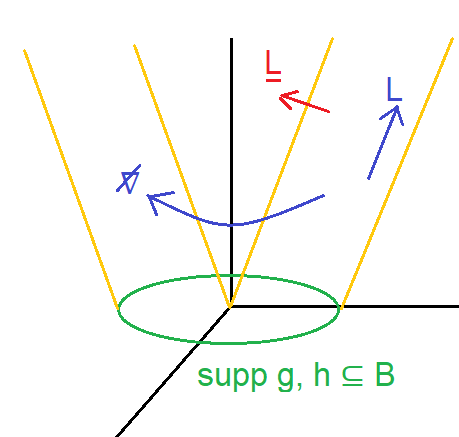
\includegraphics[scale = 0.5]{graphics/peeling}
\end{center}
Recall the radial derivative is given by $\partial_r := \frac1r \sum_j x^j \partial_j$. Define the derivatives $L$ in the $t + r$ direction, $\underline L$ in the $t - r$ direction, and $\slashed \nabla$ in the rotational direction. More concretely, 
\begin{align*}
	L
		:= \partial_t + \partial_r, \qquad
	\underline L
		:= \partial_t - \partial_r, \qquad
	\slashed\nabla_j  
		:= \partial_j  - \frac{x^j}{r} \partial_r  = \sum_{k = 1}^d \frac{x^j}{r^2} \Omega_{j, k} .
\end{align*}		
We aim to show that the ``good'' derivatives $\overline \partial \in \{ L, \slashed \nabla \}$ improve decay by $t$ in comparison to decay of the total derivative $\partial$ in Corollary \ref{cor:totaldisp}. 

\begin{theorem}[``Peeling'' for ``good" derivatives]
	Let $\phi \in C^1 (\R_t \times \R^d_x)$, then 
		\[ |\overline \partial \phi (t, x) | \lesssim \frac{1}{1 + t + r} \sum_{|\alpha| = 1} |Z^\alpha \phi (t, x)|.\] \label{thm:peel}
\end{theorem}

\begin{proof}
	We first note the case $t + r \leq 1$ is trivial since the right-hand side controls all first-order derivatives. Suppose then $t + r > 1$, and note
		\begin{align*}
			\frac{1}{t + r} \left( S + \sum_{j = 1}^d \frac{x^j}{r} H_j \right) 
				&= \frac{1}{t + r} \left( t \partial_t + \sum_{j = 1}^d x^j \partial_j + \sum_{j = 1}^d \frac{x^j}{r} \left( t \partial_j + x^j \partial_t \right) \right)\\
				&= \frac{1}{t + r} \left( (t + r)\partial_t + \sum_{j = 1}^d \frac{x^j (t + r)}{r} \partial_j\right)  = \partial_t + \partial_r = L.
		\end{align*}
	This proves the result for $\overline\partial = L$. For the rotational derivative, note the identity
		\begin{align*}
			\frac1t \left( x^j H_k - x^k H_j\right)
				&= \frac1t \left( x^j t \partial_k + x^j x^k \partial_t -  x^k t \partial_j -x^j x^k \partial_t  \right) = \Omega_{j, k}.
		\end{align*}	
	It follows from the identity above and the definition of $\slashed \nabla$ that 
		\[ |\slashed \nabla \phi| \lesssim \frac1r \sum_{j, k = 1}^d |\Omega_{j, k} \phi| \lesssim \frac1t \sum_{j = 1}^d |H_j \phi|. \]
	This proves the result for $\overline\partial =\slashed \nabla$.	
\end{proof}

\begin{corollary}
	Let $\phi$ be a solution to the $(1 + d)$-dimensional linear homogeneous wave equation (\ref{eq:linearwave}) with initial data $g, h \in C^\infty_c (B(0, R))$. Then 
		\[ |\overline \partial \phi (t, x)| \lesssim_{d, R} \frac{(1 + |t - r|)^\frac12}{(1 + t + r)^{\frac{d + 1}{2}}} \sum_{|\alpha| \leq \lfloor \frac{d + 4}{2} \rfloor} ||\partial Z^\alpha \phi ||_{L^2_x} (0). \]
\end{corollary}

\begin{proof}
	Since $Z^\alpha \phi$ also solve the linear homogeneous wave equation with initial data $Z^\alpha g, Z^\alpha h \in C^\infty_c (B(0, R))$, it follows from Corollary \ref{cor:goodlemma} that
		\[   \sum_{|\alpha| = 1} |Z^\alpha \phi (t, x)| \lesssim_{d, R}  \frac{(1 + |t - r|)^{\frac12}}{(1 + t + r)^{\frac{d - 1}{2}} } \sum_{|\alpha| \leq \lfloor \frac{d + 4}{2} \rfloor} ||\partial Z^\alpha \phi ||_{L^2_x} (0). \]
	Combining with the peeling property and rearranging finishes the proof.
\end{proof}

\begin{remark}
	Note in four-dimensional space-time $\R_t \times \R^3_x$ we only have the estimate $||\partial \phi||_{L^\infty_x} (t) \lesssim 1/t$, which is not integrable in time, however our estimate for the ``good'' derivatives $||\overline\partial \phi||_{L^\infty_x} (t) \lesssim 1/t^{3/2}$ is integrable in time.  
\end{remark}

Generally, we will not have symmetry in the quadratic non-linearity as we did when considering the equation $\Box \phi = \partial \phi \partial \phi$. Consequently, it will not be enough to place the ``good'' derivatives in $L^\infty_x$; we will also need a weighted $L^2_{t, x}$-estimate.

\begin{theorem}[Energy estimate on null cones]
	Let $\phi$ be a solution to the inhomogeneous wave equation $\Box \phi = f$ for smooth compactly supported initial data, then for $\delta > 0$,
		\[ || \nabla_{t, x} \phi ||_{L^\infty_t L^2_x (0, T)} + ||(1 + |t - r|)^{-\frac12 - \delta} \, \overline\partial \phi||_{L^2_{t, x}(0, T)} \lesssim_\delta ||\nabla_{t, x} \phi||_{L^2_x} (0) + ||f||_{L^1_t L^2_x (0, T)} . \]
		\label{thm:nullenergy}
\end{theorem}

\begin{proof}
	By the usual energy estimate, Corollary \ref{cor:energyest1}, it suffices to control the weighted $L^2$-norm of the ``good'' derivative. Recall from the proof of conservation of energy, Theorem \ref{thm:conserve}, that we can write $f \partial_t \phi$ as a divergence, 
				\begin{align*}
		f \partial_t \phi 
			&= \partial_t \left( -\frac12 (\partial_t \phi)^2 - \frac12 \sum_{j = 1}^n (\partial_j \phi)^2 \right) + \nabla_x \cdot (\partial_t \phi \, \nabla_x \phi) = \nabla_{t, x} \cdot \left( -\frac12 |\nabla_{t, x} \phi|^2, \partial_t \phi \nabla_x \phi \right).
	\end{align*}
	However, rather than integrating on $[0, T] \times \R^d_x$, we instead integrate on the null cones 
		\[C_{u_0} = \{ (t, x) :  u + u_0 = 0 \text{ and } t \in [0, T] \}, \qquad u := t - r. \]
	By a change of coordinates and $L^2_u$-integrability of $(1 + |u|)^{-\frac12 - \delta}$, we can write
		\[ ||(1 + |u|)^{-\frac12 - \delta}\, \overline\partial \phi||_{L^2_{t, x} (0, T)} \sim || (1 + |u|)^{-\frac12 - \delta}  \overline\partial \phi||_{L^2_u L^2 (C_u)} \lesssim \sup_{u} ||\overline \partial \phi ||_{L^2 (C_u)}.\]	
	It remains to control the right-hand side above. We argue as we did in the usual energy estimate, however we instead integrate over the cone region $R \subseteq [0, T] \times \R^n_x$ with boundary $\partial R = C_u + B_1 + B_2$,
	\begin{center}
		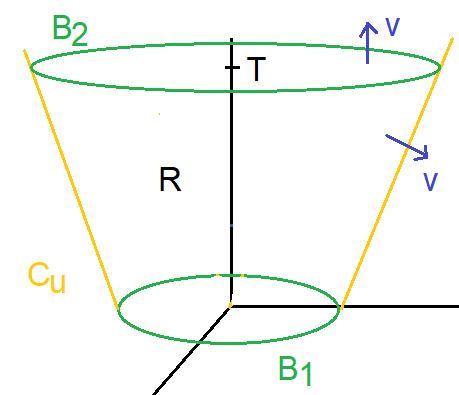
\includegraphics[scale = 0.5]{graphics/divergence}
	\end{center}
	and applying the divergence theorem gives
		\begin{align*}
			\int_R f \partial_t \phi \, dA
				& = \int_{C_{u} + B_1 + B_2} \left( -\frac12 |\nabla_{t, x} \phi|^2, \partial_t \phi \nabla_x \phi \right) \cdot \nu \, dS \\
				&= \int_{C_{u}} \left( -\frac12 |\nabla_{t, x} \phi|^2, \partial_t \phi \nabla_x \phi \right) \cdot  \left( \frac12, -\frac{x}{2|x|} \right)  dS + \frac12 || \nabla_{t, x} \phi||^2_{L^2_x (|x| \leq u)} (0) - \frac12 ||\nabla_{t, x} \phi||_{L^2_x (|x| \leq u + T)}^2 (T).
		\end{align*}	
	Observe that the integral on the null cone $C_u$ takes the form
		\begin{align*}
			\int_{C_u} \left( -\frac12 |\nabla_{t, x} \phi|^2, \partial_t \phi \nabla_x \phi \right) \cdot \left( 1, -\frac{x}{|x|} \right) dS
				&= - \frac12 \int_{C_u} \left( |\nabla_{t, x} \phi|^2  + 2 \sum_{i = 1}^n \frac{x_i}{|x|} \partial_t \phi \partial_i \phi \right) dS \\
				&= - \frac12 \int_{C_u} \left( (\partial_t \phi)^2 + (\partial_r \phi)^2 + |\slashed \nabla \phi|^2 + 2\partial_t \phi \partial_r \phi\right) dS\\
				&= - \frac12 \int_{C_u} \left(|\slashed \nabla \phi|^2 + |(\partial_t + \partial_r) \phi|^2\right)  dS\\
				&= -\frac12 \int_{C_u} \left(|\slashed \nabla \phi|^2 + |L \phi|^2 \right)  dS = - \frac12 \int_{C_u} |\overline\partial \phi|^2 dS = ||\overline \partial \phi||_{L^2 (C_u)}^2.
		\end{align*}	
	Rearranging, we conclude
			\[  \sup_{u} ||\overline \partial \phi ||_{L^2 (C_u)} \lesssim || \nabla_{t, x} \phi ||_{L^\infty_t L^2_x (0, T)}  +  ||\nabla_{t, x} \phi||_{L^2_x} (0)+ ||f||_{L^1_t L^2_x (0, T)}.\]
	This completes the proof. 	
\end{proof}

\subsection{The null condition}

\begin{definition}
	Given a matrix $Q \in \R^{d \times d}$, we say that $Q(\phi, \psi) := \sum_{j, k} Q^{j, k} \partial_j \phi \partial_k \psi$ is a \emph{null form} if it satisfies the \emph{null condition}: $\sum_{j, k} Q^{i, j} \xi_j \xi_k = 0$ whenever $\sum_{j, k} M^{j, k} \xi_j \xi_k = 0$.
\end{definition}

\begin{lemma}[Properties of null forms]
	Let $Q \in \R^{3 \times 3}$ be a null form, then the following properties hold:
	\begin{enumerate}
		\item The space of null forms is linearly generated by the Minkowski metric $M$ and the anti-symmetric matrices. 
	
		\item The null form is controlled by
					\[ |Q( \phi,  \psi)| \lesssim |\partial \phi| |\overline\partial \psi| + |\overline\partial \phi| |\partial \psi|.\]
		\item Given a commuting vector field $Z \in \{ \partial_t, \partial_j, \Omega_{jk}, H_j,  S \}$, we have
						\[ Z(Q( \phi,\psi)) = Q(Z\phi, \psi) + Q(\phi, Z \psi) + \tilde Q(\phi, \psi) \]
					for some null form $\tilde Q$. 	
	\end{enumerate}
\end{lemma}

\begin{proof}
\leavevmode
\begin{enumerate}
	\item The Minkowski metric $M$ trivially satisfies the null condition. Suppose $B^\top = - B$, then $\xi^\top B \xi = - \xi^\top B \xi$, which holds if and only if $\xi^\top B \xi = 0$. Hence, anti-symmetric matrices also trivially satisfy the null condition. Conversely, $Q$ can be written as the sum of symmetric and anti-symmetric matrices, namely
				\[ Q = \frac{Q + Q^\top}{2} + \frac{Q - Q^\top}{2} =: A + B. \]
			Then
				\[ 0 =  \xi^\top Q \xi = \xi^\top A \xi + \xi^\top B \xi = \xi^\top A \xi\]
	whenever $\xi^\top M \xi = 0$. Since $A$ is symmetric, $\xi^\top A \xi$ is a homogeneous polynomial in $\xi$ of degree $2$ which has a zero set coinciding with that of $\xi_0^2 - \sum_j \xi_j^2$. This holds if and only if $A$ is a constant multiple of $M$. 

	\item By a., it suffices to check the result for the Minkowski metric $M$ and anti-symmetric null forms $B$. The former case follows from the identity
					\[ M(\phi, \psi) = \sum_{j, k = 1}^3 M^{j, k} \partial_j \phi \partial_k \psi = \partial_t \phi \partial_t \psi - \sum_{j = 1}^3 \partial_j \phi \partial_j \psi = 2L \phi \underline L \psi + 2 \underline L \phi L \psi - \slashed \nabla \phi \cdot \slashed \nabla \psi. \]
				Each term on the right contains at least a factor of one ``good'' derivative, so the desired bound holds. 
	\item By a., it suffices to check the result for the Minkowski metric $M$ and anti-symmetric null forms $B$. This is an exercise in linear algebra and calculus. 
\end{enumerate}f\
\end{proof}

\begin{remark}
	b. guarantees that each term in the quadratic non-linearity from a null form contains at least one ``good'' derivative $\overline \partial$. By the peeling property, $|\overline \partial \phi|$ decays better than $|\partial \phi|$, and moreover the decay is integrable in time. Hence we put one of the of the two factors in the quadratic term in $L^2$ and the other in $L^\infty$. 
	
	c. guarantees that the null structure is preserved after differentiating by a commuting vector field $Z$. This allows us to extend our energy estimates on $\phi$ to $Z \phi$. 
\end{remark}

\begin{theorem}[Null structure energy estimate]
	Let $\phi$ be a solution to 
		\begin{equation}
			\Box \phi = Q(\phi, \phi) \label{eq:nullwave}
		\end{equation}
	on $\R_t \times \R^3_x$ with smooth compactly supported initial data. There exists $\epsilon > 0$ such that if
		\[ \sum_{|\alpha| \leq 5} ||\nabla_{t, x} Z^\alpha \phi||_{L^2_x} (0) \leq \epsilon \]
	then 		
		\[   \sum_{|\alpha| \leq 5} ||\nabla_{t, x} Z^\alpha \phi||_{L^2_x} (t) \lesssim   \sum_{|\alpha| \leq 5} ||\nabla_{t, x} Z^\alpha \phi||_{L^2_x} (0). \]
\end{theorem}

\begin{proof}
	We can write
		\[ \sum_{|\alpha| \leq 5} | \Box Z^\alpha \phi| \lesssim \sum_{|\beta| + |\gamma| \leq 5} |\overline \partial Z^\beta \phi| |\partial Z^\gamma \phi| \leq \left(\sum_{|\beta| \leq 2} |\overline \partial Z^\beta \phi| \right)\left( \sum_{|\gamma| \leq 5} |\partial Z^\gamma \phi| \right) + \sum_{|\beta| \leq 5, \, |\gamma| \leq 2} |\overline \partial Z^\beta \phi \partial Z^\gamma \phi|, \]
	where the first inequality holds since the commuting vector fields preserve the null structure. For the first term on the right, we put $\overline \partial$ in $L^\infty_x$ and apply Theorem \ref{thm:peel} the peeling property, and the Klainerman-Sobolev inequality, and we place $\partial$ into $L^2_x$, which gives us
		\[\left|\left| \left(\sum_{|\beta| \leq 2} |\overline \partial Z^\beta \phi| \right)\left( \sum_{|\gamma| \leq 5} |\partial Z^\gamma \phi| \right) \right|\right|_{L^1_t L^2_x(0, T)}\lesssim \int_0^T \frac{1}{(1 + t)^{\frac32}} \left( \sum_{|\alpha| \leq 5} || \partial Z^\alpha \phi ||_{L^2_x} \right)^2 dt \leq 2  \left( \sum_{|\alpha| \leq 5} || \partial Z^\alpha \phi ||_{L^\infty_t L^2_x (0, T)} \right)^2  \]
	For the second term, we apply Cauchy-Schwartz in $t$ to put $\overline\partial$ into weighted $L^2_{t, x}$ and $\partial$ into weighted $L^2_t L^\infty_{x}$,
		\begin{align*}
			\sum_{|\beta| \leq 5, \, |\gamma| \leq 2}  ||\overline \partial Z^\beta \phi \partial Z^\gamma \phi ||_{L^1_t L^2_x (0, T)} 
				&\leq \left(\sum_{|\beta| \leq 5}  || (1 + |t - r|)^{-\frac{1 + \delta}{2}} \overline \partial Z^{\beta} \phi ||_{L^2_{t, x} (0, T)}\right) \left(\sum_{|\gamma| \leq 2} || (1 + |t - r|)^{\frac{1 + \delta}{2}} \partial Z^\gamma \phi ||_{L^2_t L^\infty_x (0, T)} \right).
		\end{align*}
	For the weighted $L^2_t L^\infty_{x}$ term above, we apply Klainerman-Sobolev,
		\[ \left(\sum_{|\gamma| \leq 2} || (1 + |t - r|)^{\frac{1 + \delta}{2}} \partial Z^\gamma \phi ||_{L^2_t L^\infty_x (0, T)} \right) \lesssim \int_0^T \frac{1}{(1 + t)^{2-\delta}} \sum_{|\alpha| \leq 5} ||\partial Z^\alpha \phi||_{L^2_x} dt \lesssim_\delta \sum_{|\alpha| \leq 5} ||\partial Z^\alpha \phi||_{L^\infty_t L^2_x (0, T)}  \]
	where the last inequality follows from integrability of $1/(1 + t)^{2 - \delta}$ for $0 < \delta < 1$. Collecting our results, it follows from Theorem \ref{thm:nullenergy} the energy estimate on the null cone, applied to $Z^\alpha \phi$ that 
		\begin{align*}
			\sum_{|\alpha| \leq 5} ||\nabla_{t, x} Z^\alpha \phi ||_{L^2_x} 
				&+ ||(1 + |t - r|)^{-\frac{1 + \delta}{2}} \overline\partial Z^\alpha \phi||_{L^2_{t, x}} \\
				&\leq C\sum_{|\alpha| \leq 5} ||\nabla_{t, x} Z^\alpha \phi||_{L^2_x} (0) +C \left( \sum_{|\alpha| \leq 5} || \nabla_{t, x} Z^\alpha \phi ||_{L^\infty_t L^2_x (0, T)} \right)^2 \\
				&\qquad + C \left(\sum_{|\alpha| \leq 5}  || (1 + |t - r|)^{-\frac{1 + \delta}{2}} \overline \partial Z^{\alpha} \phi ||_{L^2_{t, x} (0, T)}\right) \left(\sum_{|\alpha| \leq 5} ||\nabla_{t, x} Z^\alpha \phi||_{L^\infty_t L^2_x (0, T)}  \right)
		\end{align*}	
	for some implicit constant $C > 0$ depending only on $k = 5$ and $0 < \delta < 1$. We conclude the result by a bootstrap argument; let $B \geq 2 (C + 1)$ and suppose $T \geq 0$ such that	
		\[ \sum_{|\alpha| \leq 5} ||\nabla_{t, x} Z^\alpha \phi ||_{L^\infty_t L^2_x (0, T)} +  ||(1 + |t - r|)^{-\frac{1 + \delta}{2}} \, \overline\partial Z^\alpha \phi||_{L^2_{t, x}(0, T)} \leq  B\sum_{|\alpha| \leq 5} ||\nabla_{t, x} Z^\alpha \phi||_{L^2_x} (0). \]
	The result clearly holds for $T  = 0$ by choice of $B \geq 1$, so the base case of our continuous induction on time is satisfied. We aim to prove a stronger bound than the one assumed. The previous two inequalities imply 
		\begin{align*}
			\sum_{|\alpha| \leq 5} ||\nabla_{t, x} Z^\alpha \phi ||_{L^2_x} (t)  + ||(1 + |t - r|)^{-\frac{1 + \delta}{2}} \overline\partial Z^\alpha \phi||_{L^2_{t, x}}
				&\leq C\sum_{|\alpha| \leq 5} ||\nabla_{t, x} Z^\alpha \phi||_{L^2_x} (0) +C B^2 \left( \sum_{|\alpha| \leq 5} || \nabla_{t, x}Z^\alpha \phi ||_{L^2_x} (0) \right)^2.
		\end{align*}	
	To complete the argument, it suffices to show the right-hand side satisfies the bound
		\[ C\sum_{|\alpha| \leq 5} ||\nabla_{t, x} Z^\alpha \phi||_{L^2_x} (0) +C B^2 \left( \sum_{|\alpha| \leq 5} || \nabla_{t, x} Z^\alpha \phi ||_{L^2_x} (0) \right)^2 \leq \frac12 B \sum_{|\alpha| \leq 5} ||\nabla_{t, x} Z^\alpha \phi||_{L^2_x} (0). \]
	Rearranging, it is equivalent to show
		\[ CB^2 \sum_{|\alpha| \leq 5} ||\nabla_{t, x} Z^\alpha \phi||_{L^2_x} (0) \leq \frac12 B - C. \]
	Given data sufficiently small, i.e. $\epsilon \ll 1$, completes the proof. 			
\end{proof}
